\section{Präliminarien}
\subsection{Komplexe Zahlen}
Wenn man mit den Zahlen arbeitet, die jeder kennt aus dem Alltag, bekommt man Probleme, wenn man die Wurzel einer negativen Zahl zieht. Jedoch haben Mathematiker im 16. Jahrhundert eine Lösung dafür entdeckt, indessen wir unseres Zahlensystems erweitern mit dem imaginären Zahlen und mit der imaginären Einheit i. Addieren und Subtrahieren zweier imaginären Zahlen funktioniert genau gleich wie, wenn man mit einer Variabel rechnet, jedoch beim Multiplizieren, Dividieren und beim somit entstehenden Rechnen mit Potenzen muss man aufpassen, denn es gilt für $n \in \mathbb{Z}$:
% Gleichunugen
\begin{align*}
 \text{i}^{4n} &= 1 \\
\text{i}^{4n+1} &= \text{i} \\
\text{i}^{4n+2} &= -1 \\
\text{i}^{4n+3} &= -\text{i} 
\end{align*}
%Weiter im Text
Dies ist dann zu ersetzen. Hier sieht man gut, dass die imaginären Zahlen zu reellen Zahlen werden können, wie es auch andersrum war. Wenn man nun eine imaginäre Zahl $\text{i}b$ mit einer reellen Zahl $a$ zusammenaddiert, bekommt man eine komplexe Zahl  $a+\text{i}b$ mit dem Realteil $a$ und dem Imaginärteil $\text{i}b$. $a$ und $b$ sind hier reelle Zahlen.
\\
Nun merkt man, dass diese Zahl vergleichbar ist mit einem Vektor, denn um die Zahl darstellen zu können benutzt man die 2-Dimensionale komplexe Ebene, daraus schliesst sich das komplexe Zahlen 2-Dimensional sind. Hieraus sieht man, dass beim Multiplizieren und Potenzieren es Wort Wörtlich Komplex wird. Schaut man dies Auf der komplexe Ebene an, fängt der Punkt sich scheinbar unkontrolliert herumspringen, folgt jedoch weiterhin logischen Regeln, beim Quadrieren verschiebt sich der Punkt in die positive Richtung, Gegenuhrzeigersinn. Ebenfalls kann, da die Zahl vergleichbar ist mit einem Vektor, den Absoluten Wert der komplexen Zahl $c$ bestimmt  werden:
\[|c| = \sqrt[2]{a^2+b^2} \]

\subsection{Fraktale Geometrie}
\subsubsection{Allgemein}
Um zum Buddhabrot zu kommen, brauchen wir noch einen weiteren Begriff zu klären, das Fraktal.\\ Würde bei einem 3$n$ grossem Strich der mittlere Teil fehlen, stattdessen den Rest eines gleichseitigen Dreiecks dort stehen, hat man eine Kochkurve. Ich werde man nun in die $n$ grosse Striche die gesamte Kochkurve einfügen, muss man dies ab nun immer wieder machen, sodass es schwer vorstellbar wird. Wenn man jedoch nun in die Kockurve reinzoomt, findet man die Kochkurve immer wieder. Ein rekursives Bild oder eben ein Fraktal. Man definiert nun das Fraktal als eine Figur, bei der sehr oft Selbstähnlichkeit auffindbar ist (das heisst, dass das gesamte Fraktal oder Teile davon mehrfach im Fraktal vorkommen) und das Fraktal selbst eine gebrochene und somit keine ganzzahlige Dimension besitzt.\\
\\
In der Abbildung \ref{fig:Kochkurve} ist die Entstehung der Kochkurve zu sehen.

\begin{figure}[h]
    \centering
    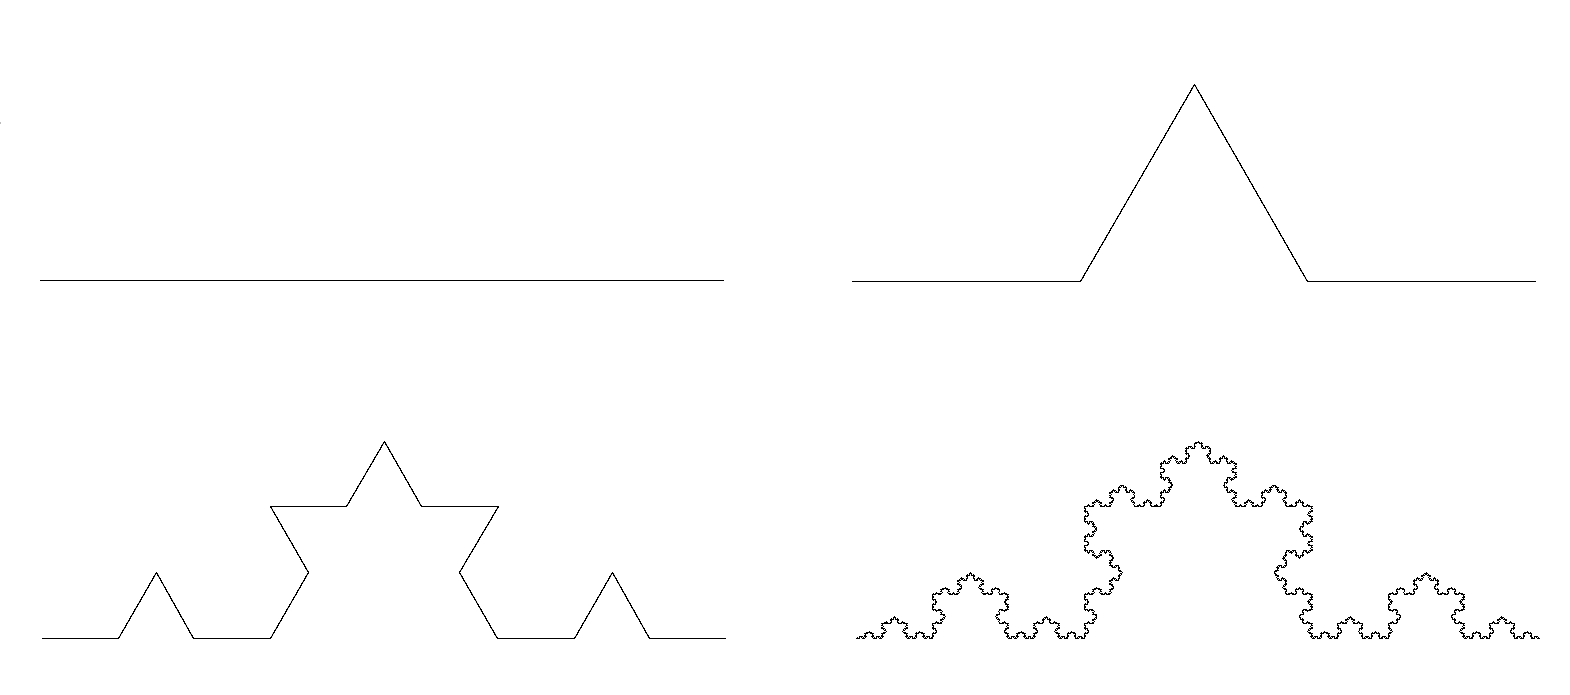
\includegraphics[width=.5\textwidth]{Pictures/Kochkurve.png}
    \caption{Kochkurve}
    \label{fig:Kochkurve}
\end{figure}

\subsubsection{Mandelbrotmenge}
Die nach dem Mathematiker Benoît B. Mandelbrot (*20.11.1924; †14.10.2010) bennanten Menge ($\mathbb{M}$), beinhaltet jede Zahl $c$ die nicht bestimmt divergiert im unendlichen für folgende Folge:
\begin{align*}
z_0&=0\\
z_{n+1}&=z^2_n+c\\
\end{align*}